\section{GPT-J}
\label{sec:gpt_j}

The generative model used to create the tickets is GPT-J, an open source 6 billion parameter, autoregressive text generation model trained on The Pile dataset released by EleutherAI. \\
The Pile dataset\cite{gao2020pile} is an 825 GiB English text corpus composed by 22 diverse subsets, which can be grouped in 5 categories:
\begin{itemize}
    \item Academic ( \textit{ArXiv}, \textit{PubMed Central}, ... )
    \item Internet ( \textit{Wikipedia}, \textit{StackExchange}, ... )
    \item Prose ( \textit{Bibliotik}, ... )
    \item Dialogue ( \textit{Subtitles}, ... )
    \item Misc ( \textit{Github}, ... )
\end{itemize}
\subsection{Parameters}
\label{sec:parameters}
The parameters used for the generation of the next token are:
\begin{itemize}
    \item \textit{min\_length}: minimum number of words created by a round of gpt generation
    \item \textit{max\_length}: maximum number of words created by a round of gpt generation.  
    \item \textit{top\_k}: the k most likely next words are filtered and the probability mass is redistributed among only these k words. It helps the model not to go off-topic.
    \item \textit{top\_p}: the next words are sampled from the smallest possible set of words whose cumulative probability exceeds the probability p. Compared to \textit{top\_k}, in this case the size of the set of possible next token is not fixed. In practice, usually \textit{top\_k} and \textit{top\_p} are used together.
    \item \textit{temperature}: the value $T$ used to module the logits distribution. The higher the value of $T$, the higher the entropy of the logits distribution will be. In other words, tokens with an high probability will be less probable and tokens with a low probability will be more probable.
    \begin{equation*}
        p_i = \frac{exp(x_i/T)}{\sum_j exp(x_j/T)}   
    \end{equation*}
    \item \textit{repetition\_penalty}: the parameter $\theta$ for repetition penalty. 1.0 means no penalty \\
    Given a list of generated tokens $G$, 
     \begin{equation*}
        p_i = \frac{exp\left(\frac{x_i}{T \cdot I(i \in G)}\right)}{\sum_j exp\left(\frac{x_j}{T \cdot I(j \in G)}\right)}
    \end{equation*}
    \begin{center}
    $I(c) = \theta$ if $c$ is True else 1
    \end{center}    
    So the logits distribution of the token change based on if the token has already been generated before.

    \item \textit{length\_penalty}: \textit{length\_penalty} $>$ 0 promotes longer sequences, while \linebreak 
    \textit{length\_penalty} $<$ 0 encourages shorter sequences.

    \item \textit{no\_repeat\_ngram\_size}: If set to an integer $>$ 0, all ngrams of that size can only occur once \\
    Ex: \textit{no\_repeat\_ngram\_size} = 2 \\
    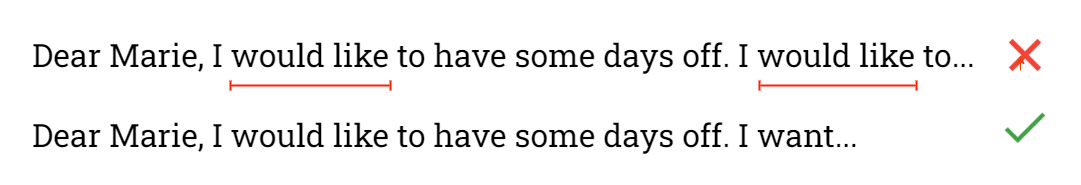
\includegraphics[width=0.94\textwidth]{images/no_ngram_thesis.drawio.png}

    \item \textit{num\_beams}: Number of beams for beam search. They beams are the number of 'paths' that are considered when choosing the next token. Even if a token is not the one with the highest probability, it can be chosen as the next token if the complete sentence is considered as more probable than the alternatives. \\
    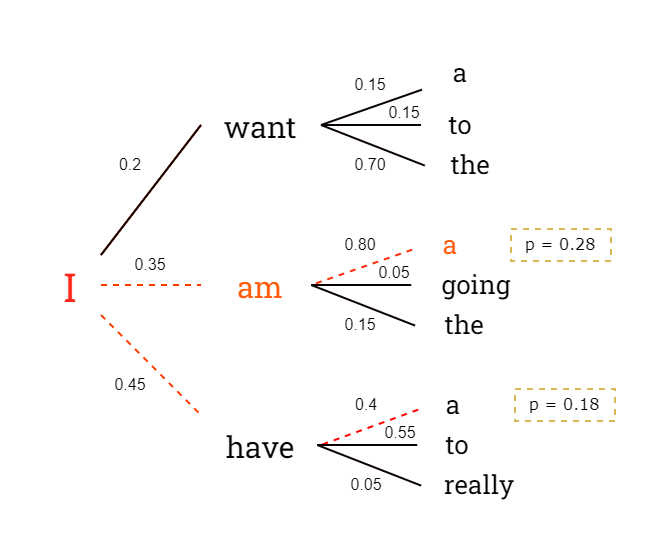
\includegraphics[width=0.6\textwidth]{images/num_beams.drawio.png}

    \item \textit{do\_sample}: If set to `False` greedy decoding is used ( the most probable token is always chosen). Otherwise, sampling is used ( the next token is chosen sampling from the distribution of possible next tokens )
    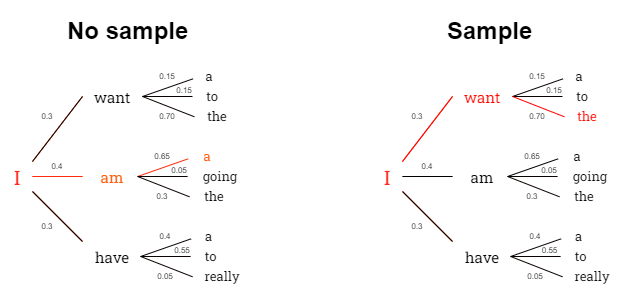
\includegraphics[width=0.90\textwidth]{images/do_sample.drawio.png}

    \item \textit{bad\_words}: List of words that are not allowed to be generated by the model.
    \item \textit{force\_words}: List of words that must be generated in the generation.
    
\end{itemize}
The default values assigned to the parameters used are shown in \autoref{table:parametersGPTJTable}, however the application is set up in order to being able to apply different parameters at each run.

\begin{table}[h] 
\centering
\begin{tabular}{|l|l|}
\hline
Parameter          & Value \\ \hline
min length         & 0    \\ 
max length         & 50    \\ 
top k              & 50    \\
top p              & 0.85  \\
repetition penalty & 1.2   \\
temperature        & 1     \\
length penalty     & 1     \\
no repeat ngram size     & 0     \\
num beams &  1 \\
do sample & True \\
bad words & [\space] \\
force words & [\space] \\ \hline
\end{tabular}
\caption{Parameters of GPT-J model}\label{table:parametersGPTJTable}
\end{table}
\subsection{Architecture}
The GPT architecture is based on the original Transformers paper. The original architecture introduced two types of transformers blocks: the encoder block and the decoder block. \\
The encoder block converts an input sequence of tokens into a sequence of embedding vectors, whereas the decoder takes the output of the encoder and generate iteratively an output sequence of tokens. \\
GPT is pre-trained by predicting the next word based on the previous ones. \\
GPT is decoder-only, which means that is assembled only by a stack of decoder blocks. Each decoder block is composed by:
\begin{itemize}
    \item \textbf{Normalization Layers}: a normalization layer \cite{ba2016layer} normalize all inputs of a neural network across their features. It has been shown that Layer normalization enables smoother gradients, faster training, and better generalization accuracy \cite{xu2019understanding}

    $x$: data sample \\
    $d$: dimension of data sample \\
    $y$: output of LayerNorm \\
    $\epsilon$: small number added for stability

    \begin{equation*}
        u = \frac{1}{d}\sum_{i=1}^{d}x_i 
    \end{equation*}
    \begin{equation*}
        \sigma^2 = \frac{1}{d}\sum_{i=1}^{d}(x_ - ui)^2
    \end{equation*}
    \begin{equation*}
        \hat{x_i} = \frac{x_i - u}{\sqrt{\sigma^2 + \epsilon}}
    \end{equation*}
    \begin{equation*}
        y = \gamma\hat{x_i} + \beta
    \end{equation*}

    where $\gamma$ and $\beta$ are parameters that the model learns.
    \item \textbf{Masked Self-Attention Layer}: attention is a mechanism that allows neural networks to assign a different amount of weight to each token in a sequence and process each token as a weighted average of all other tokens. \\
    In practice three matrixes are calculated:
    \begin{itemize}
        \item $Q$ (Query): the representation of the current token
        \item $K$ (Key): the representation of all the other tokens, which are matched with the current token
        \item $V$ (Value): the representation of all the words, used for the weighted-average
    \end{itemize}
    The $Q$, $K$ and $V$ matrixes are initialized as:
    \begin{itemize}
        \item $Q$ = $W_qX + b_q$ 
        \item $K$ = $W_kX + b_k$ 
        \item $V$ = $W_vX + b_v$
    \end{itemize}
    where $X$ is the input matrix and the other matrixes are randomly initialized and learned by the model.
    Finally, the attention score is calculated with
    \begin{equation*}
        Attention(Q,K,V) = softmax \left(\frac{QK^T}{\sqrt{d}}\right)V
    \end{equation*}
    where $d$ is a normalization factor equivalent to the embeddings' dimension \\
    The masked self-attention is a modified version of self-attention where all the tokens that appear after the current one are set to $0$, in order not to let the model being influenced by any information regarding the tokens at the next positions. This is fundemental when training generative models such as GPT, whose scope is to predict the successive tokens.
    \begin{equation*}
        Attention(Q,K,V) = softmax\left(\frac{QK^T + Mask}{\sqrt{d}}\right)V
    \end{equation*}

    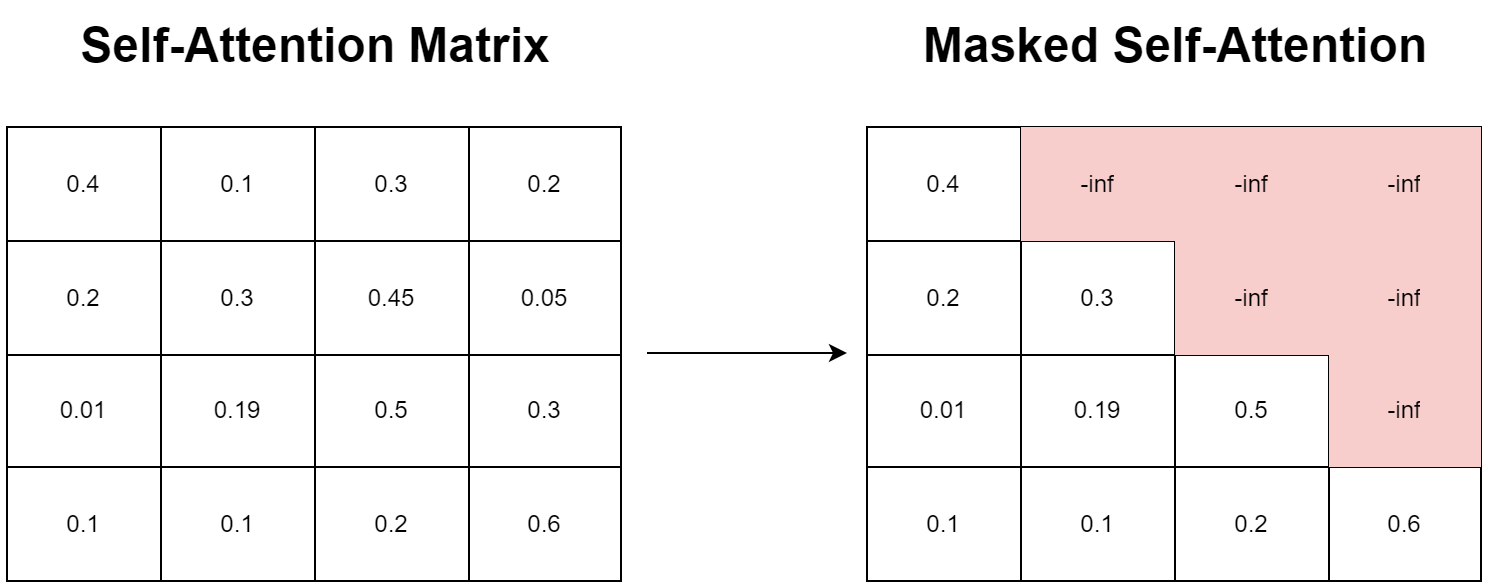
\includegraphics[width=0.90\textwidth]{images/masked_self_attention.drawio.png}

    \item \textbf{Feed Forward Neural Network Layer}: Used to add non-linearity to the transformer block
\end{itemize}

\begin{figure}[h] 
    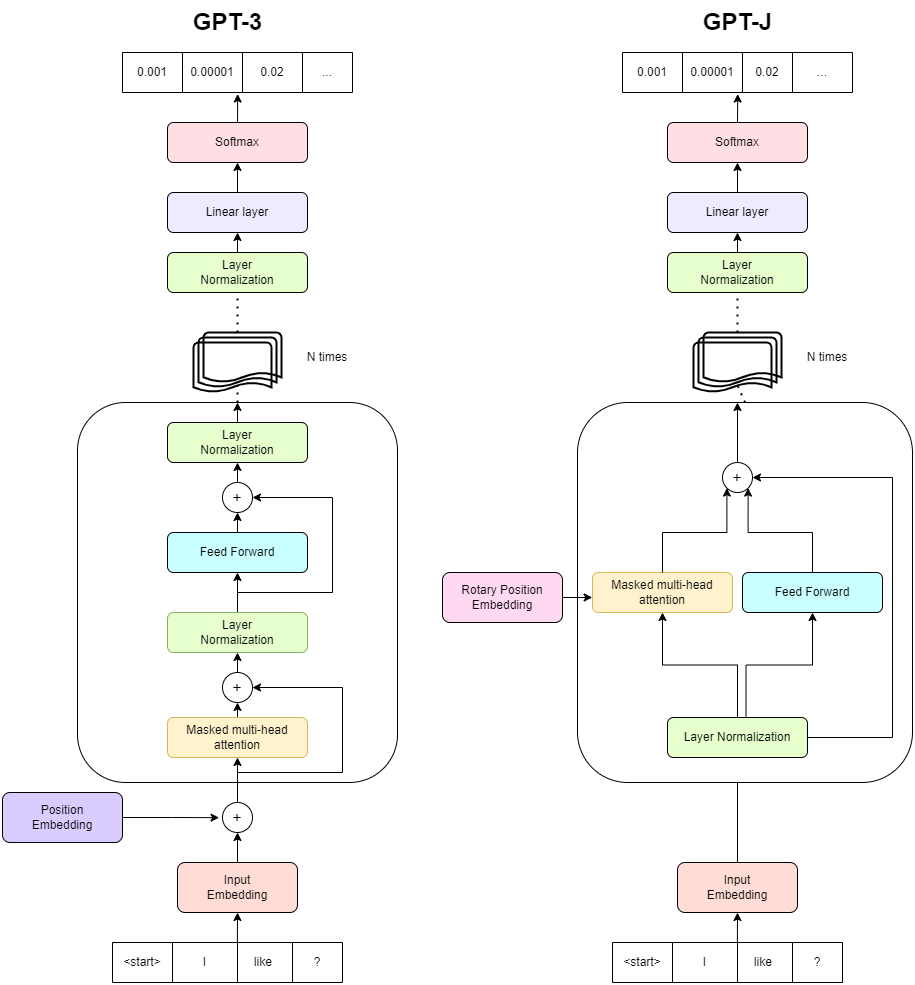
\includegraphics[width=\textwidth]{images/gptJ_vs_gpt_architecture.drawio.png}
    \caption{GPT-3 and GPT-J architectures compared}
    \label{fig:gpt-architectures}
\end{figure}    

\begin{figure}[h] 
    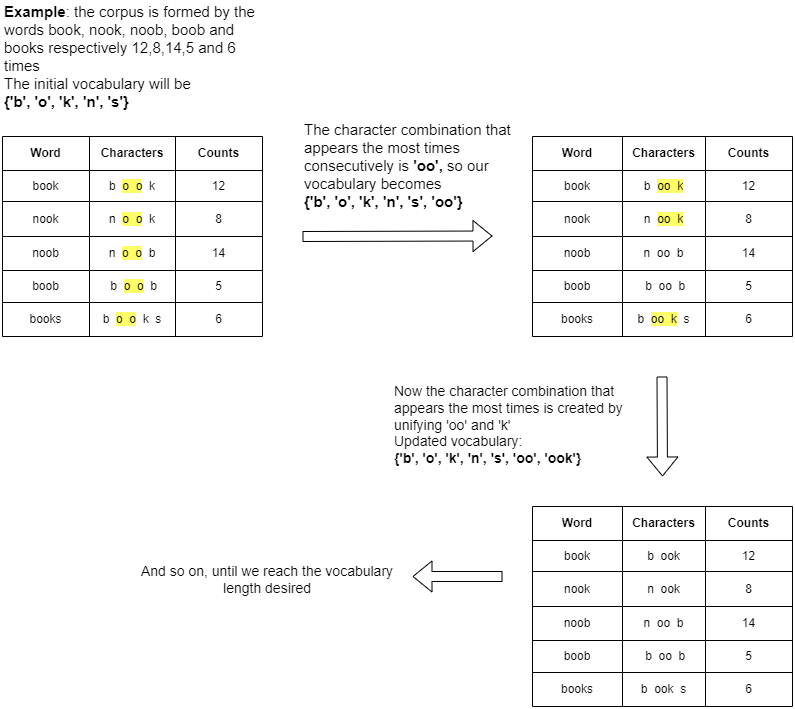
\includegraphics[width=\textwidth]{images/byte_pair.drawio.png}
    \caption{Byte-Pair Encoding Tokenization Example}
    \label{fig:Byte_Pair_Encoding}
\end{figure}    


GPT models use a Byte-Pair Encoding tokenization. The Byte-Pair Encoding algorithm starts by building a vocabulary with all the single characters of the corpus we are training on. Then, at each step of the algorithm, the two tokens which appear consecutevily the most in the words of the corpus are unified and create a new token. This process continue until the desired vocabulary lenght is satisfied. An example taken from the site \cite{byte-pair-encoding} is shown in the \autoref{fig:Byte_Pair_Encoding}


Compared to GPT-3, GPT-J\cite{gptj} has two minor architectural differences  ( shown in \autoref{fig:gpt-architectures}):
\begin{itemize}
    \item Rotary Embedding
    \item The attention layer and the feedforward layer in parallel for decreased communication
\end{itemize}

\subsubsection{Rotary Position Embedding}
Position embeddings are used to infer the notion of position to the model, which does not have any sense of position for each token. In other words, using the attention mechanism each token "match" with the other tokens in the same manner, not considering where if the other token is located right after the current one or if it is at the end of the sentence. Position embeddings are used to add to the model this sense of position. \\ Rotary position embedding has been introduced by Su et al.\cite{su2021roformer}, it is a novel method that unifies absolute and relative approaches to position embeddings. \\
The typical approach, which is also used by GPT-3, is to use a sinusoidal embedding, which is defined as
\begin{equation*}
    \begin{cases}
        p_{1,2t} = sin(k/10000^{2t/d}) \\
        p_{1,2t+1} = cos(k/10000^{2t/d}) 
    \end{cases}
\end{equation*}
where $p_{1,2t}$ is the $2^{th}$ element of the d-dimensional vector $p_i$
RoPE instead proposes to incorporate the relative position information by multiplying the context representation with the sinusoidal functions instead of directly adding them. \\
If we define 
\begin{equation*}
    \begin{split}
        q_m = f_q(x_m, m) \\
        k_n = f_k(x_n, n) 
    \end{split}    
\end{equation*}

where $f_q$ and $f_k$ are functions that incorporate the $m^{th}$ and $n^{th}$ positions respectively to the vector embeddings $x_m$ and $x_n$ to produce the query and key vectors, we can require the inner product of the query $q_m$ and $k_n$ to be formulated by a function $g$ that depends only on the word embeddings $x_m$, $x_n$ and their relative position $m - n$
\begin{equation*}
    \langle f_q(x_m, m) \: , \: f_k(x_n, n) \rangle = g(x_m,x_n,m-n)
\end{equation*}
In the simplest case $d=2$, $f_{\{q,k\}}$ are defined as
\begin{equation*}
    f_{(\{q,k\}, \{m,n\})} = (W_{\{q,k\}}x_{\{m,n\}})e^{i\{m,n\}\theta}
\end{equation*}
and therefore we obtain
\begin{equation*}
    g(x_m, x_n, m - n) = Re[(W_qx_m)(W_kx_n)^Te^{i(m-n)\theta}]
\end{equation*}
which preserves the relative positional information of the word embeddings. This equation is used when calculating the self-attention, which will become
\begin{equation*}
    Attention(Q,K,V) = softmax\left(\frac{g(x_m, x_n, m - n)}{\sqrt{d}}\right)V
\end{equation*}
This equation can be generalized for $d > 2$, as shown in the original paper. \\
In the end, incorporating the RoTE is pretty straightforward, you just have to rotate the word embedding by a multiple of its position index. \\
According to the researchers that published GPT-J\cite{rope-eleutherai}, using RoTE leads to a faster convergence of training and validation losses and a lower overall validation loss.

\noindent
\begin{minipage}{\linewidth}
    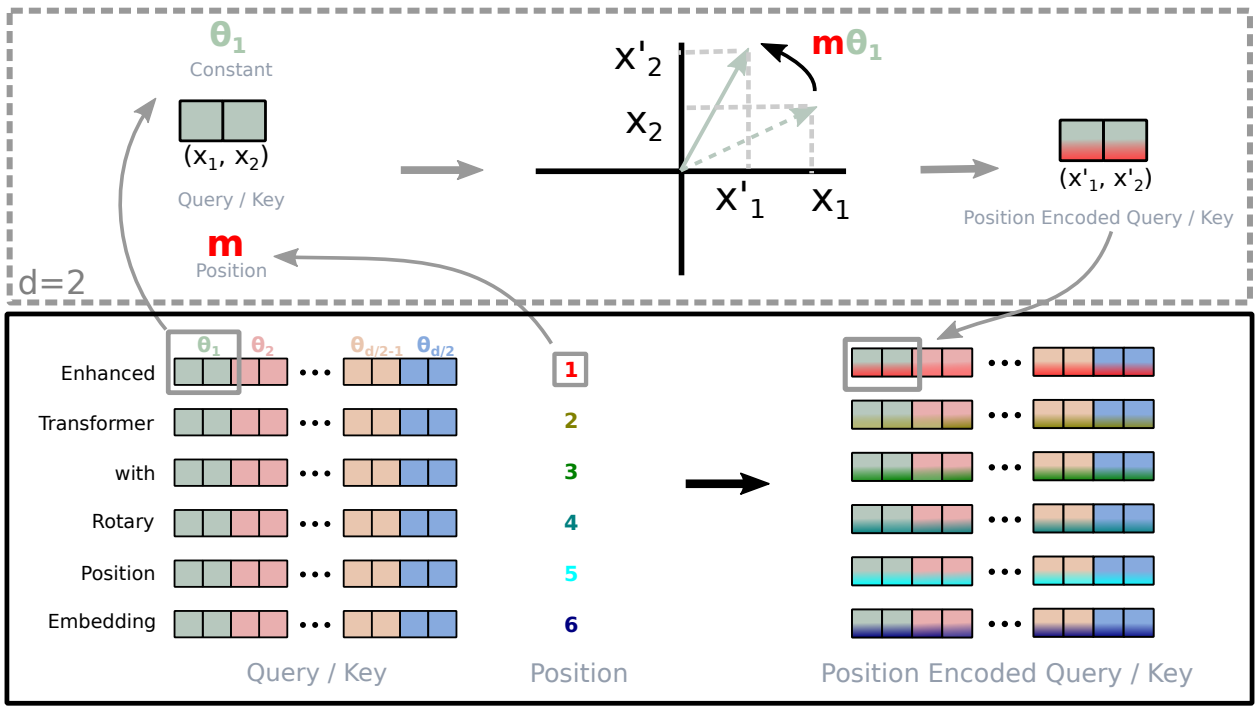
\includegraphics[width=\linewidth]{images/rotary_embedding_from_paper.PNG}
    \captionof{figure}{Implementation of RoPE, Image taken from original paper\cite{su2021roformer}}
\end{minipage}%